\documentclass[letterpaper,10pt]{article}

\usepackage{titling}
\usepackage{listings}
\usepackage{url}
\usepackage{setspace}
\usepackage{subfig}
\usepackage{sectsty}
\usepackage{pdfpages}
\usepackage{colortbl}
\usepackage{multirow}
\usepackage{multicol}
\usepackage{relsize}
\usepackage{amsmath}
\usepackage{wasysym}
\usepackage{fancyvrb}
\usepackage{amssymb}
\usepackage{ifsym}
\usepackage{amsmath,amssymb,amsthm,graphicx,xspace}
\usepackage[titlenotnumbered,noend,noline]{algorithm2e}
\usepackage[compact]{titlesec}
\usepackage{XCharter}
\usepackage[T1]{fontenc}
\usepackage{tikz}
\usetikzlibrary{arrows,automata,shapes,trees,matrix,chains,scopes,positioning,calc}
\tikzstyle{block} = [rectangle, draw, fill=blue!20, 
    text width=2.5em, text centered, rounded corners, minimum height=2em]
\tikzstyle{bw} = [rectangle, draw, fill=blue!20, 
    text width=4em, text centered, rounded corners, minimum height=2em]

\definecolor{namerow}{cmyk}{.40,.40,.40,.40}
\definecolor{namecol}{cmyk}{.40,.40,.40,.40}

\let\LaTeXtitle\title
\renewcommand{\title}[1]{\LaTeXtitle{\textsf{#1}}}


\newcommand{\handout}[5]{
  \noindent
  \begin{center}
  \framebox{
    \vbox{
      \hbox to 5.78in { {\bf ECE356: Database Systems } \hfill #2 }
      \vspace{4mm}
      \hbox to 5.78in { {\Large \hfill #4  \hfill} }
      \vspace{2mm}
      \hbox to 5.78in { {\em #3 \hfill} }
    }
  }
  \end{center}
  \vspace*{4mm}
}

\newcommand{\lecture}[3]{\handout{#1}{#2}{#3}{Lecture #1}}
\newcommand{\tuple}[1]{\ensuremath{\left\langle #1 \right\rangle}\xspace}

\addtolength{\oddsidemargin}{-1.000in}
\addtolength{\evensidemargin}{-0.500in}
\addtolength{\textwidth}{2.0in}
\addtolength{\topmargin}{-1.000in}
\addtolength{\textheight}{1.75in}
\addtolength{\parskip}{\baselineskip}
\setlength{\parindent}{0in}
\renewcommand{\baselinestretch}{1.5}
\newcommand{\term}{Winter 2018}

\singlespace


\begin{document}

\lecture{ 9 --- Database Design: Normalization }{\term}{Jeff Zarnett}

\section*{Database Design}
So far, we learned the syntax to create tables, and how to turn modelling diagrams into tables and all the various bits and pieces about how modelling diagrams work. The modelling diagrams give us some guidance and tell us about wrong ways to represent the data, but we don't yet have enough guidance as to what is correct. If we do a good job the relation will be in a \textit{normal form}. Yes, \textit{a} normal form... there are several.

An example from~\cite{dsc} gives us an opportunity to do something wrong and show bad design: if we combine instructor (having the attributes id, name, department, salary) with department (having an id, faculty, budget) then our combined table means one larger relation replaces two smaller ones. This isn't total nonsense because instructors do have a relationship with a department, but is this a good way to model the data? Intuition might tell you no, but think about why. In the combined relation, if there are two instructors, say, Sedra and Smith, both members of department of electrical \& computer engineering, in both tuples there will be an entry for the budget of the department. The budget data is duplicated and risks becoming inconsistent.

Our intuition may tell us this is bad, but we would like a way to express it formally. Informally the rule is that each value of department name corresponds to at most one budget. The formal description is a \textit{functional dependency} and it is written \textit{dept\_name} $\rightarrow$ \textit{budget}. A functional dependency specified that if there is a schema that consists just of the attributes for department name and budget, then the department name attribute could be the primary key~\cite{dsc}. Combining instructor and department breaks this rule, because we have duplicate entries for department and therefore this can't work.

The functional dependency shows us that data is duplicated and that indicates that we need to split the combined relation in a process called \textit{decomposition}.

The previous example is very egregiously and obviously wrong, making it simple to identify that there is a problem. In reality, a database will have many more tables and it will be harder to find out what the functional dependencies are, but there is an algorithm for that which will be covered soon enough.

Another example from~\cite{dsc} shows us that decomposition on its own is not always good: we should split up things that don't belong together, but it is possible to go overboard. If the relation is \textit{employee( ID, name, street, city, province, postalcode )}, we might think that we can decompose this into two schemas: \textit{employee(ID, name), address(name, street, city, province, postcode)}. Does this work? No -- two employees could have the same name and that is likely in the real world, as some names are extremely popular. 

If instead of defining the address relation to be based on name, we could use the ID instead, and it would work: \textit{employee(ID, name), address(employeeID, street, city, province, postcode)}. This is an acceptable decomposition and we call it \textit{lossless} because no information is lost. The first attempt at this caused a loss of information (if two employees have the same name, there is the possibility of confusion), so it is called a \textit{lossy} decomposition. We do not perform lossy decompositions.

\subsection*{Atomic Domains and the First Normal Form}

Our E-R model allows attributes to be non-atomic, that is to say, divisible. If a course code is ``ECE356'', that attribute is non-atomic because it can be divided into two parts, the ``ECE'' (department) and ``356'' (course number) components. The same is true of something like an address: ``48 Main Street Southwest Unit 2A'' might be the street attribute, but that is divisible into several parts. Those are non-atomic attributes values. If the domain is indivisible units, e.g., an integer, it is atomic.

A relation $R$ is said to be in the \textit{first normal form} (abbreviated as 1NF) if the domain of all attributes of $R$ are atomic. If some attribute is not atomic, then we could subdivide it to put it into 1NF. Instead of course being ``ECE356'' we could split  it up into department ``ECE'' and number ``356''. The primary key could still be composed of those two elements, mind you.

Does this mean that a string (varchar) attribute can never be atomic, as one may take a subset? No, what really matters is how they are used in the database. If the application logic requires breaking up the attribute for some reason, then it is non-atomic. The ``ECE356'' example is not atomic because there are situations where you would want to subdivide this. To answer the question ``how many courses in the Winter 2018 term are ECE courses?'', we need to look at all course codes and figure out which ones begin with ``ECE''. If employee numbers are generated in the format ``AA1234'' and can never be subdivided (e.g., the first two letters don't indicate anything like department) then they are atomic. 

More than this, though, we don't like set-valued attributes. If we wanted to model all the departments that belong to a faculty, what we don't want is for the faculty tuple to have an attribute called departments which then contains multiple elements... For example, Engineering is a faculty, and the list of departments would be ECE, MME, SYDE, etc. This would not be in the first normal form, because the attribute of departments could be split up into each department. This can cause confusion and redundancy. What about Software Engineering? It belongs to the faculty of Engineering and Math... Data could be related.

\subsection*{Decomposition with Functional Dependencies}

The schema that we create is supposed to model entities and their relationships in the real world. The real world understanding tells us important information about how the data should be modelled: students have a student ID number and the student ID number is unique. If the database does not represent that information in some way, we have done something wrong. The real world constraints may be represented as a key or as a functional dependency.

The schema is just the data model, and we care if the data in the tables conforms to the constraints. If the data in the table meets all the real-world constraints, that instance of the relation is called a \textit{legal instance}. If all tables in the database are a legal instance of that relation, then we can say the instance of the database is a legal instance of the database schema~\cite{dsc}.

A \textit{superkey} is a subset $K$ of a relation $R$ if, in any legal instance of $R$, for all pairs, of tuples $t_{1}$ and $t_{2}$ in the instance of $r$, if $t_{1} \neq t_{2}$ then $t_{1}[K] \neq t_{2}[K]$~\cite{dsc}. This is to say that no two tuples in a legal instance of the relation may have the same values the subset of attributes $K$, or if you prefer, the attributes in $K$ allow a tuple in the relation to be uniquely identified.

Suppose that attributes $\alpha$ and $\beta$ are part of a relation $r$. A functional dependency $\alpha \rightarrow \beta$ is satisfied if for all pairs of tuples $t_{1}$ and $t_{2}$ such that $t_{1}[\alpha] = t_{2}[\alpha]$ it is the case that $t_{1}[\beta] = t_{2}[\beta]$. If this functional dependency holds on every legal instance of the relation, we can say the functional dependency holds on the schema~\cite{dsc}.

If it helps you to imagine this, a functional dependency tells us that for a given value of $x$, we know what the value of $y$ will be. In this way it is like a function in math, if we know the value of $x$ we know the value of $f(x)$ (namely, $y$). And most importantly, for every value of $x$ there is at most one $y$. 

We can say that $K$ is a superkey of $R$ if the functional dependency $K \rightarrow R$ holds on this instance of the relation. That means, formally, that if $t_{1}[K] = t_{2}[K]$ then it means $t_{1} = t_{2}$ because a superkey identifies a tuple uniquely.

Functional dependencies are used for both design and verification purposes. We use them in the design process to identify and record the constraints that our database schema should be designed around. They will be used as a way to decide what entities should be formed and how their relationships to others appear. And when we have a set of functional dependencies, we can use them to verify if an instance of the database is legal; that is, check if all constraints are satisfied. If the answer is yes, then we say the set of functional dependencies holds.
 
\begin{center}
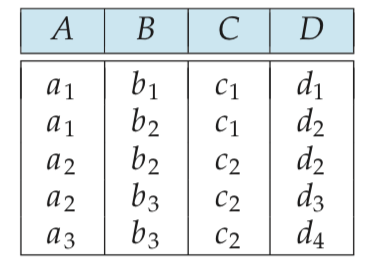
\includegraphics[width=0.2\textwidth]{images/fd-1}\\
A sample relation with dummy data~\cite{dsc}
\end{center}

In the sample data above, we can identify the dependency $A \rightarrow C$ because for each tuple where the value of $A$ is $a_{1}$, the value of $C$ is the same ($c_{1}$), where $A$ is $a_{2}$, $C$ is $c_{2}$, and where $A$ is $a_{3}$, $C$ is $c_{2}$. That is, by knowing the value of $A$ we can know the value of $C$. We can also see that $C \rightarrow A$ does not hold.

You are probably thinking that this relation has only five tuples in it and it may just be a coincidence that $A \rightarrow C$ holds on this relation. And that is entirely possible. Our data is observational here, not prescriptive. Without knowing a bit about what $A$ and $C$ are we don't know if it should be the case. Based on what we have here we can only verify if certain functional dependencies hold, if they are provided. 

There are also \textit{trivial} functional dependencies because they are always true and not even the smallest bit interesting. The functional dependency $A \rightarrow A$ is an example of a trivial dependency, and not very useful. A formal definition of a trivial relation is that $\alpha \rightarrow \beta$ is trivial if $\beta$ is a contained within $\alpha$ (in set thinking)~\cite{dsc}.

Functional dependencies can be transitive: if $A \rightarrow B$ and $B \rightarrow C$, then $A \rightarrow C$. For each $A$ there can be only one value of $B$ and for that value of $B$ there is only one corresponding $C$. If a set of functional dependencies is $F$, the notation that includes all of these implied dependencies is $F^{+}$, the \textit{closure} of $F$~\cite{dsc}.

\subsection*{Boyce-Codd Normal Form}

The \textit{Boyce-Codd Normal Form}, known as BCNF, eliminates all redundancy that can be found using functional dependencies (but it does not eliminate all redundancy). A schema $R$ is in BCNF with respect to a set of functional dependencies in $F$, if, for all functional dependencies in $F^{+}$ of the form $\alpha \rightarrow \beta$ either (1) the functional dependency is trivial, or (2) $\alpha$ is a superkey for schema $R$~\cite{dsc}. A database is in BCNF if all its relations are in BCNF.

Calling back to the earlier example where we looked at merging instructor and relation, we can see that this is not in BCNF fairly easily. A department has a budget, yes, but in this relationship a the department name is not a superkey because we had two entries (Sedra, Smith) that were in the same department and those had the same budget. A department cannot have two budgets.

Our real-world understanding tells us that there is a dependency that says a department has a budget, and only one budget (even if the department chair would like to have the sum of the budgets...). That tells us there should exist a functional dependency. Given that a functional dependency should exist, check it against he conditions for BCNF. It is not trivial, nor is department name a superkey for this combined relation.

The general approach to decompose things that are not in BCNF from~\cite{dsc}. If it is not in BCNF there is at least one nontrivial functional dependency $\alpha \rightarrow \beta$ where $\alpha$ is not a superkey for $R$. Then we need to split up $R$ into two relations: (1) $(\alpha \cup \beta)$ and (2) $(R - (\beta - \alpha))$. The rule is stated in this way because sometimes we need to have attributes that appear on both sides of the arrow. We may need to repeat that process on one of the new relations until it is in BCNF.

\paragraph{Dependency Preservation.} Avoiding duplication of data is not our only goal in a database design. Constraints also need to be checked. Although we have not yet seen how joins are performed, or why they are expensive (really), for now we should just understand that joins are expensive and we would like to avoid them. Checking if a constraint is satisfied may require a computationally expensive join if the relations are in BCNF.

Consider an example from~\cite{dsc}: the previous relationship between student and advisor has been altered. Now, if a student wishes to have multiple advisors, that is permitted, but the student may only have at most one advisor from a given department. How realistic this scenario may be is not really the goal.

\begin{center}
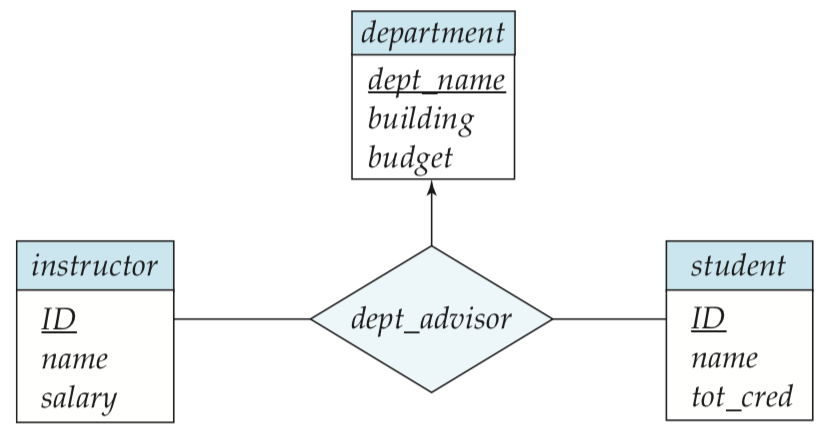
\includegraphics[width=0.5\textwidth]{images/advise-3}\\
E-R diagram for ternary advisor-student-department relationship~\cite{dsc}
\end{center}

The relation in the diagram above to represent \textit{dept\_advisor} will contain three attributes, all of which are primary keys in the other relations: \textit{(student\_id, instructor\_id, dept\_name)}. Based on what we know, the functional dependencies are \textit{instructor\_id} $\rightarrow$ \textit{dept\_name} (an instructor belongs to one department). and \textit{student\_id, dept\_name} $\rightarrow$ \textit{instructor\_id} (a student has at most one advisor per department). 

This design is not in BCNF, because \textit{instructor\_id} is not a superkey. An instructor ID alone is not enough to identify the relationship, because multiple students can be advised by the same individual. So we need to perform the decomposition procedure and that will produce two relations: \textit{(student\_id, instructor\_id)} and \textit{(instructor\_id, dept\_name)}.

Those are in BCNF, but it is difficult to verify the constraint that requires us to verify that each triple of \textit{(student\_id, instructor\_id, dept\_name}) is unique. That is because performing this check requires a join on the two relations in the previous paragraph. That is computationally expensive, as we will soon see. 

Because it is now hard to check this dependency, the design is said to not be \textit{dependency preserving}. It is not that it is impossible to check the dependency, although the terminology might seem to imply that data is somehow lost. It is not lost, just harder to check and verify.

\subsection*{Third Normal Form}
The Third Normal Form, or 3NF, is weaker than BCNF that allows dependencies to be preserved. Now wait, you say, third normal form? What happened to the second normal form? Is BCNF the second normal form? No, it is separate from BCNF. A table is in the second normal form if it is in the first normal form and all non-key columns are dependent on the table's primary key~\cite{secnorm}. The second normal form is not especially popular and is mostly here for completeness. It is the third normal form that we are interested in. 
 
The 3NF rules are a small modification of the BCNF rules. In particular, we would like to allow some nontrivial functional dependencies whose left side (the $\alpha$) is not a superkey. 

A schema $R$ is in 3NF with respect to a set of functional dependencies in $F$, if, for all functional dependencies in $F^{+}$ of the form $\alpha \rightarrow \beta$ one of the following holds: (1) the functional dependency is trivial, or (2) $\alpha$ is a superkey for schema $R$~\cite{dsc}, or (3) Each attribute $A$ in $\beta - \alpha$ is contained in a candidate key for $R$. Any one of those conditions suffices. Remember also that a candidate key is a minimal superkey. Note also that the third condition does not mean a single candidate key must contain all attributes in $\beta - \alpha$; as long as each attribute appears in at least one candidate key~\cite{dsc}.

Remember that a schema that is in BCNF would satisfy case 1 or 2 for each of the functional dependencies, so anything in BCNF is already in 3NF. 3NF, however, is slightly less restrictive and allows functional dependencies that are not permitted in BCNF, so something in 3NF may or may not be in BCNF.

Recall: the relation in the diagram in the previous subsection to represent \textit{dept\_advisor} contains three attributes, all of which are primary keys in the other relations: \textit{(student\_id, instructor\_id, dept\_name)}. Based on what we know of the functional dependencies, this relation is already in 3NF. The step we took to do the decomposition to BCNF is unnecessary here if we can accept 3NF. There are tradeoffs, but we can come back to what those are...

How do we know the new definition of \textit{dept\_advisor} is in 3NF? We know that the current definition has a functional dependency that does not meet condition 1 or 2, otherwise it would be in BCNF. So the rule we will check is the third rule and we'll find that this is valid because \textit{instructor\_id} is contained in a candidate key: \textit{(student\_id, instructor\_id)} is a candidate key, because it is minimal and sufficient to identify any row. If the student with ID x999chan is supervised by Professor Sedra, we have enough information to figure out that the department is ECE.

\subsection*{Higher Normal Forms}

\bibliographystyle{alphaurl}
\bibliography{356}


\end{document}
